\toclesssection{SCP 032 - Titania's Prisons}
\addcontentsline{toc}{section}{SCP 032 - Titania's Prisons}

\textbf{Item \#:} SCP-032

\textbf{Object Class:} Safe

\begin{figure}[h]
\begin{center}
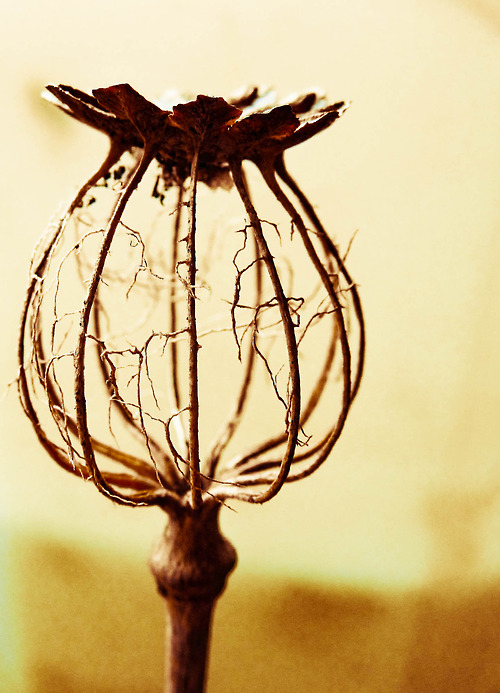
\includegraphics[scale=0.35]{scp/032.jpg}
\linebreak Container of SCP-032-1 after its release.
\end{center}
\end{figure}

\textbf{Special Containment Procedures:} SCP-032 is to be kept in a locked greenhouse, at a temperature of 24° Celsius. Portions of SCP-032 are to be removed only with permission from the Site Director.

\textbf{Description:} SCP-032 is a cluster of flowers, all with identical appearances, contained in a single clay pot. Examination of SCP-032 has revealed these plants do not share DNA with any other plant species found on earth, despite their resemblance to [REDACTED]. The blossoms of SCP-032 have been revealed, on closer examination, to contain a variety of small life forms, with one being contained in the center of each blossom. Upon removal of one of these blossoms, the entity (hereby referred to SCP-032-1) inside of it came to life, and was subsequently interviewed. SCP-032-1 died of unknown causes shortly after the interview.

SCP-032 was obtained by an undercover operative in London, England, from an antiquities shop.
\newpage
\textbf{Addendum:}

\textbf{Interview 032-1}

Interviewed: SCP-032-1

Interviewer: Dr. \censor{XXXXX}

Foreword: SCP-032-1 was previously contained inside SCP-032. The goal of the interview was to establish who SCP-032-1 was, why they were in SCP-032, and what SCP-032 was.

$<$Begin Log$>$

"Dr. \censor{XXXXX}:" What is your name?

"SCP-032-1:" I am Neusara. Where am I?

"Dr. \censor{XXXXX}:" Why were you inside the flower?

"SCP-032-1:" The Queen had placed me there, because I had been caught by a mortal.

"Dr. \censor{XXXXX}:" The Queen?

"SCP-032-1:" You know of her. I do not wish to speak her name. It could summon her. …Please, I don't understand, what has happened? How did you find me?

"Dr. \censor{XXXXX}:" We do not know who you are speaking about? Who is this Queen?

"SCP-032-1:" But, all mortals know her name…unless…Oh. Oh no.

*SCP-032-1 began to cry, and would not respond to further questioning*

$<$End Log$>$

Closing Statement: SCP-032-1 died an hour after the interview. Autopsy was unable to determine cause of death, the medical examiner stating that "Her heart just stopped."